\documentclass[12pt, letterpaper]{article}
\usepackage{graphicx}

\title{Pymagicc: A Python wrapper for the simple climate
model MAGICC}
\author{S M Arifuzzaman}
\date{August 7, 2020}

\begin{document}

\maketitle

\section{Introduction}
Pymagicc\footnote{https://github.com/openscm/pymagicc} is a Python wrapper around the reduced complexity climate model MAGICC6\footnote{http://magicc.org/}.  
Pymagicc runs on Windows, macOS and Linux and simplifies usage of the model by
utilising DataFrames from the Pandas library (McKinney 2010) as a data structure for
emissions scenarios. To read and write the text-based MAGICC configuration and output
files in the Fortran Namelist format Pymagicc utilizes the f90nml library (Ward 2017). All MAGICC model parameters and emissions scenarios can thus easily be modified through
Pymagicc from Python. MAGICC (Model for the Assessment of Greenhouse Gas Induced Climate Change) is widely used in the assessment of future emissions pathways in climate policy analyses, e.g. in the Fifth Assessment Report of the Intergovernmental Panel on Climate Change (IPCC 2014). Many Integrated Assessment Models (IAMs) utilize MAGICC to model the
physical aspects of climate change. It has also been used to emulate complex atmosphereocean general circulation models (AOGCM) from the Coupled Model Intercomparison
Projects.

In this project, I use one of preloaded RCP (Representative Concentration Pathway) scenario to create 1 plot, and another plot was created using all four (4) scenarios RCP. 
 


\section{Methods}

\subsection{Dataset}
The dataset used for this demonstration is the demo data provided by MAGICC under RCPs scenarios. The RCPs describe 4 different scenarios based on different assumptions about population, economic growth, energy consumption and sources and land use over this century. These scenarios are preloaded in Pymagicc, each RCP scenario describe alternative trajectories for carbon dioxide emissions and the resulting atmospheric concentration from 2000 to 2100.



\section{Pymagicc for RCPs data visualization}

\subsection{Global Mean Temperature Projection}
I have created a python script named Plot1\_GlobalMeanTemperatureProjection  to visualize the Mean temperature projection from the year of 1850 to 2100. After running this script it draws a plot. 

\subsection{horizontal\_section() method}
The horizontal\_section method inside the oceanspy.plot module plots horizontal section plot. I created a GenerateTempwithDepth.py file that downloads the example data file provided by OceanSpy and then uses the method horizontal\_section() to draw a plot where temperature is plotted where the horizontal axis is longitude and vertical axis is latitude, the contour channel is controlled using the depth column of the dataset. 


\section{Results}
\begin{figure}
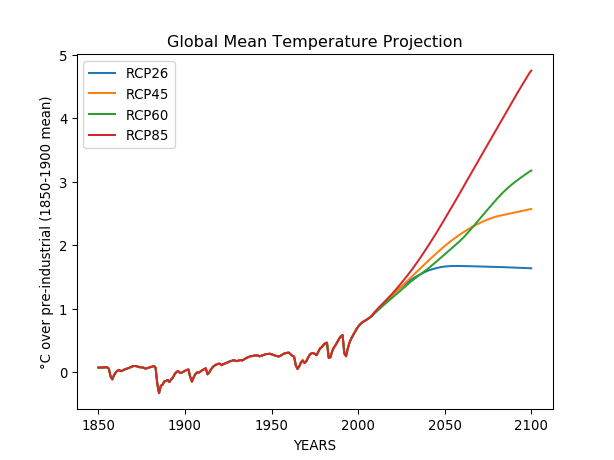
\includegraphics[width=1\textwidth]{Plot1_GlobalMeanTemperatureProjection.png}
\caption{Global Mean Temperature Projection}
\label{fig:Plot1_GlobalMeanTemperatureProjection}
\end{figure}


The first figure successfully generated. It can be seen that on figure \ref{fig:Plot1_GlobalMeanTemperatureProjection}, along with the plot some data with legends. Also from the plot, it can be observed that global temperature increasing rapidly after the year 2000. 












\section{Conclusions}
Still in progress...

\end{document}